\documentclass[11pt]{article}
\usepackage[margin=1in]{geometry}
\usepackage[T1]{fontenc}
\usepackage{lmodern}
\usepackage{amsmath}
\usepackage{booktabs}
\usepackage{graphicx}
\usepackage{float}
\usepackage[authoryear,round]{natbib}
\usepackage[hidelinks]{hyperref}
\usepackage{enumitem}
\setlist{itemsep=2pt, topsep=4pt}
% Primitive \input, so generated table rows can be followed by \bottomrule.
\makeatletter\newcommand\inputrows[1]{\@@input #1 }\makeatother

\title{Early Detection of Alzheimer's Disease:\\From Logistic Regression to XGBoost\\[4pt]\large Revised edition}
\author{Haocheng Sun \and Chi Zhang \and Xile Chen}
\date{STA314 course project, Kaggle team ``Vegetable Dogs''\\
Submitted December 2024; revised October 2026 by Haocheng Sun}

\begin{document}
\maketitle

\begin{abstract}
We compare logistic regression, random forest and XGBoost for classifying Alzheimer's disease (AD)
from demographic, lifestyle, clinical and cognitive features in a public \emph{synthetic} dataset of
1,504 labelled records. All models are tuned and evaluated with the same nested cross-validation, so
the reported scores are not inflated by hyperparameter selection. XGBoost reaches an accuracy of
$0.957 \pm 0.009$ and an AUC of 0.958, against $0.833 \pm 0.023$ and 0.897 for logistic regression.
The gap has a simple cause: the risk of AD in these data changes in steps at cut-offs of the three
strongest predictors (MMSE, functional assessment and ADL), which trees represent directly and a linear
logistic model cannot. At a screening threshold chosen to catch at least 90\% of AD cases, XGBoost keeps
a specificity of 0.977 versus 0.715 for logistic regression. This revision corrects
several errors in the submitted 2024 report, which are listed in Section~\ref{sec:changes}.
\end{abstract}

\section{Introduction}

Alzheimer's disease is a progressive neurodegenerative disease and the most common cause of dementia,
accounting for an estimated 60--70\% of cases \citep{rosselli2022culture}. It is characterized by the
gradual loss of cognitive, behavioural and functional abilities, associated with the deposition of
beta-amyloid plaques and tau proteins in the brain. Its causes are not fully understood, but genetic,
environmental and lifestyle factors all contribute: the 2020 Lancet Commission identified 12 modifiable
risk factors, including hypertension, diabetes, physical inactivity and smoking, that together account
for around 40\% of dementia worldwide \citep{livingston2020dementia}. Around 50 million people lived with
dementia in 2020, a number projected to reach 152 million by 2050 \citep{livingston2020dementia}.

Despite its prevalence, AD is often diagnosed late or not at all, particularly in low- and
middle-income countries \citep{lazarova2023detection}, and most diagnoses happen at moderate to severe
stages, when treatment is least effective \citep{li2024intelligentdiagnosisalzheimersdisease}. Cheap
screening tools that can be used in the community, without specialist staff, could help refer the right
people for clinical assessment. For such a tool the most costly error is a \emph{missed} case, so a
screening model must be judged by its recall (sensitivity), not only by its accuracy.

This project asks how well standard classifiers can identify AD from routinely collected features,
and how an interpretable model (logistic regression) compares with tree ensembles (random forest and
XGBoost). Because the dataset is synthetic (Section~\ref{sec:data}), the results describe how the data
generator relates the features to the diagnosis; they are an exercise in model building and evaluation,
not clinical evidence.

\section{Data}\label{sec:data}

\subsection{Source}
We use the Alzheimer's Disease Dataset of \citet{elkharoua2024dataset}, published on Kaggle under a
CC~BY~4.0 licence. According to its author the dataset \emph{is synthetic and was generated for
educational purposes}. It contains 2,149 records; the course competition provided 1,504 labelled records
for training (\texttt{data/train.csv}) and 645 unlabelled records (\texttt{data/test.csv}) whose
predictions were scored on Kaggle, split into a public and a private part.

\subsection{Variables}
After dropping the identifier \texttt{PatientID} and the constant column \texttt{DoctorInCharge}
(``XXXConfid'' for every record), there are 32 predictors:
\begin{itemize}
  \item 15 continuous: Age, BMI, AlcoholConsumption, PhysicalActivity, DietQuality, SleepQuality,
  SystolicBP, DiastolicBP, four cholesterol measures, the Mini-Mental State Examination score (MMSE,
  0--30), FunctionalAssessment (0--10) and Activities of Daily Living (ADL, 0--10). Lower MMSE,
  FunctionalAssessment and ADL scores indicate more impairment.
  \item 2 nominal: Ethnicity and EducationLevel, with four levels each.
  \item 15 binary: Gender, Smoking, family history, five comorbidities (cardiovascular disease, diabetes,
  depression, head injury, hypertension) and seven symptoms (MemoryComplaints, BehavioralProblems,
  Confusion, Disorientation, PersonalityChanges, DifficultyCompletingTasks, Forgetfulness).
\end{itemize}
The target \texttt{Diagnosis} is 1 for a diagnosis of AD and 0 otherwise; 532 of the 1,504 training
records (35.4\%) are positive.

\subsection{Exploratory analysis}
There are no missing values. The predictors are almost uncorrelated with each other: the largest
absolute pairwise correlation is 0.082 (BMI and CholesterolHDL). In particular, MemoryComplaints,
DifficultyCompletingTasks and Forgetfulness have pairwise correlations between $-0.01$ and $0.06$.
The labelled and unlabelled records also look alike: no feature differs in mean by more than 0.10
standard deviations between the two.

Five features carry almost all of the signal (Figure~\ref{fig:assoc}): FunctionalAssessment ($r=-0.37$),
ADL ($-0.33$), MemoryComplaints ($0.30$), BehavioralProblems ($0.24$) and MMSE ($-0.24$). No other
feature has an absolute correlation with the diagnosis above 0.07.

\begin{figure}[tbp]
  \centering
  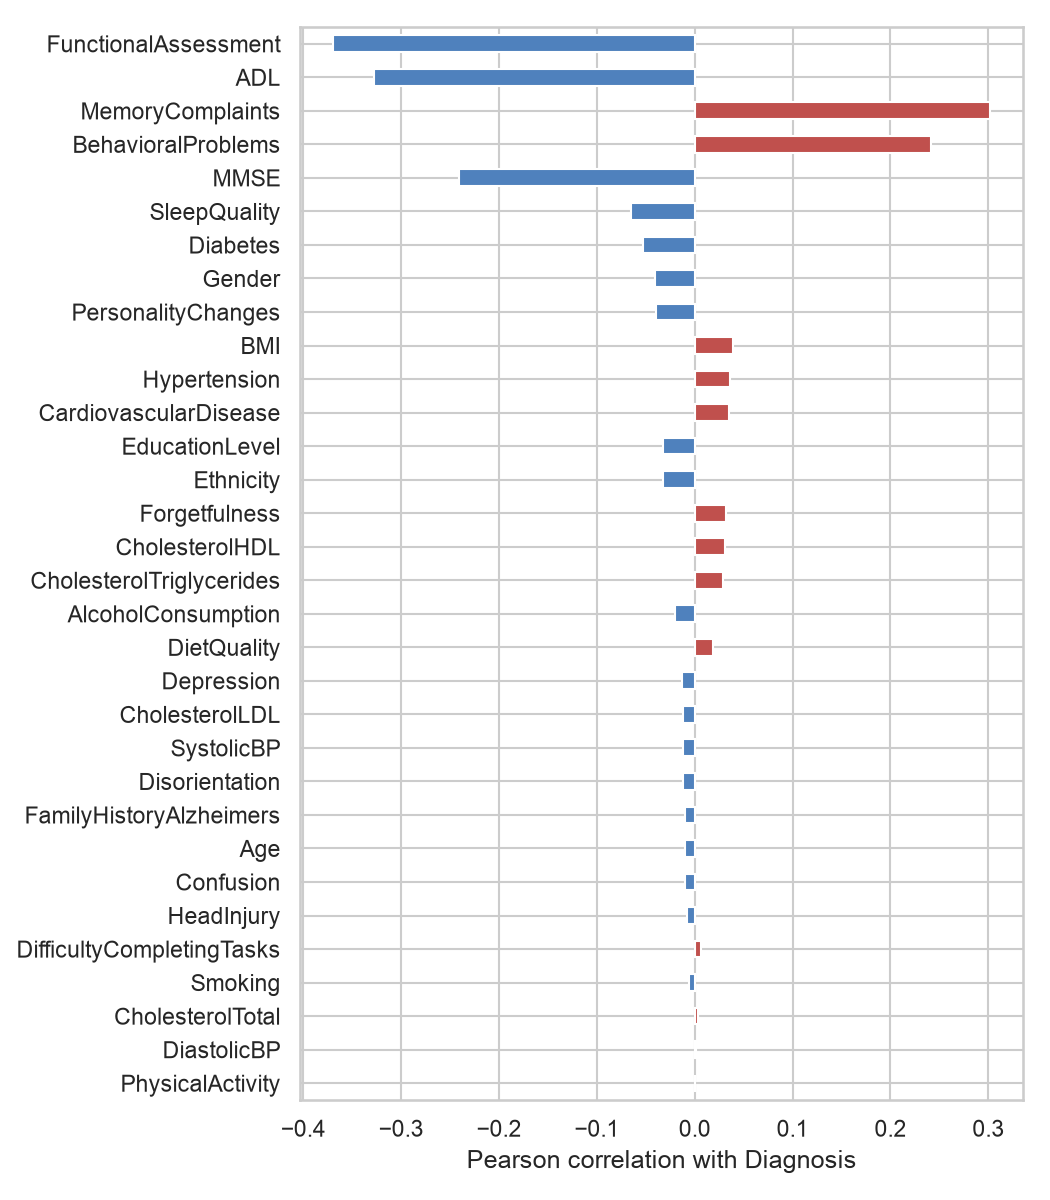
\includegraphics[width=0.46\linewidth]{figures/eda_target_correlation.png}
  \caption{Correlation of each predictor with the diagnosis (training data).}
  \label{fig:assoc}
\end{figure}

Correlation understates how strongly the three continuous scores matter, because their effect is
step-like (Figure~\ref{fig:steps}). The share of AD diagnoses is 42.5\% among records with MMSE below
24 but 3.6\% at 24 or above; it is 55.8\% versus 16.3\% on either side of FunctionalAssessment~$=5$,
and 53.0\% versus 16.9\% on either side of ADL~$=5$. Within each side the rate is roughly flat. This
shape matters for model choice: a logistic regression that is linear in the features can only fit a
smooth S-shaped change, while a decision tree can split exactly at the cut-off.

\begin{figure}[H]
  \centering
  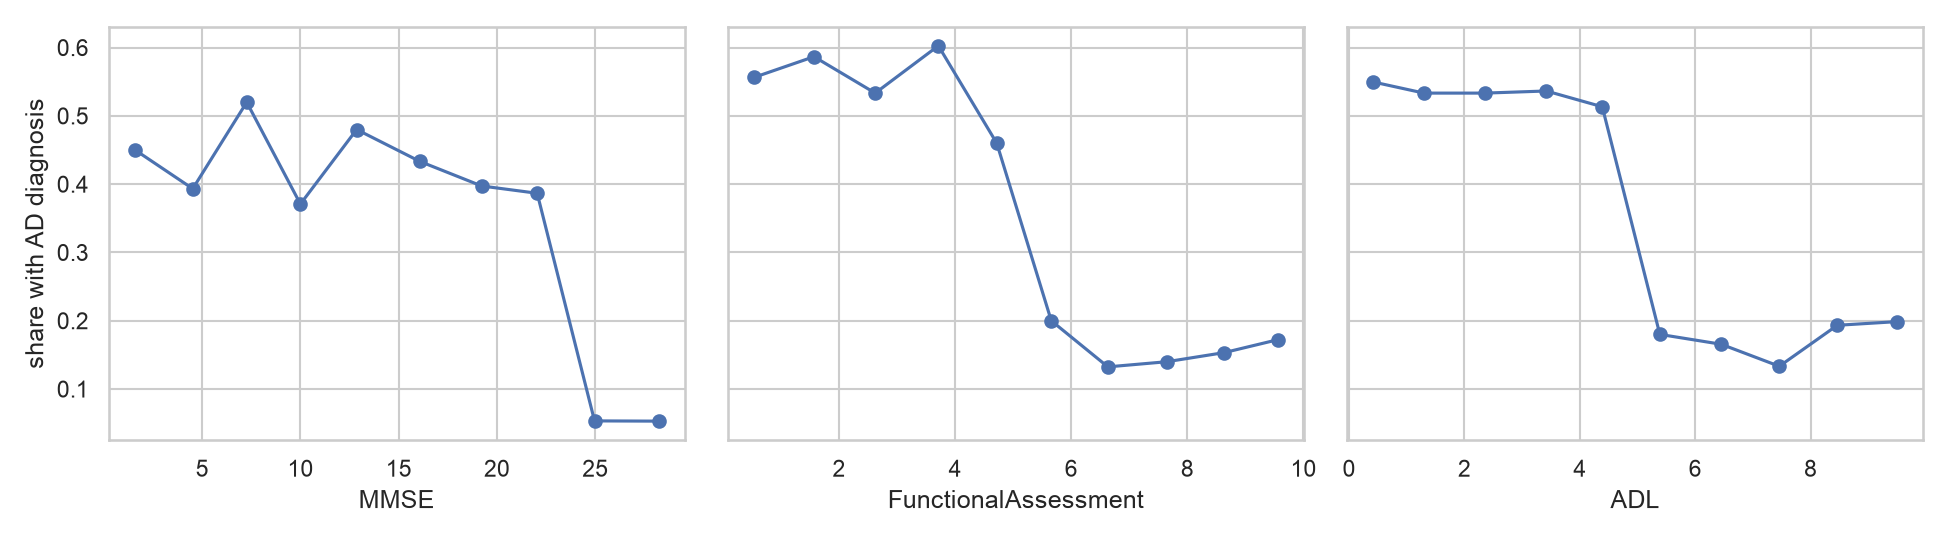
\includegraphics[width=\linewidth]{figures/eda_binned_rates.png}
  \caption{Share of AD diagnoses by decile of MMSE, FunctionalAssessment and ADL.}
  \label{fig:steps}
\end{figure}

\section{Methods}\label{sec:methods}

\subsection{Preprocessing}
Continuous features are min-max scaled to $[0,1]$, the two nominal features are one-hot encoded (first
level dropped) and binary features are used as they are. The preprocessing is part of each model's
pipeline, so it is fitted on training folds only. Tree models are unaffected by the scaling; it is kept
so that all models see identical inputs.

\subsection{Models}
\begin{itemize}
  \item \textbf{Logistic regression} with an L1 (lasso) or L2 (ridge) penalty; the penalty type and its
  strength $C \in [10^{-2}, 10^{2}]$ (25 log-spaced values) are tuned by grid search.
  \item \textbf{XGBoost} \citep{chen2016xgboost}: randomized search over 60 candidates for the number of
  trees (50--600), maximum depth (2--8), learning rate (0.01--0.3, log scale), row subsampling
  (0.6--1.0), column subsampling (0.5--1.0) and minimum child weight (1--10).
  \item \textbf{Random forest}: randomized search over 40 candidates for the number of trees (100--600),
  maximum depth (4--20 or unlimited), minimum leaf size (1--10) and features per split.
\end{itemize}
All models are implemented with scikit-learn \citep{pedregosa2011scikit} and xgboost; candidates are
ranked by cross-validated accuracy, the metric of the Kaggle competition.

\subsection{Evaluation}
Choosing the best of many hyperparameter settings on a validation set and then reporting the score on
that same set overstates performance, because the winner is partly chosen for fitting the noise of that
particular split \citep{varma2006bias, cawley2010overfitting}. We therefore use \emph{nested}
cross-validation. The 1,504 records are split into five stratified outer folds. For each outer fold, the
whole tuning procedure above is run on the other four folds using an inner stratified 5-fold
cross-validation; the selected model is refitted on those four folds and evaluated once on the held-out
fold. We report the mean and standard deviation over the five outer folds. All models use the same
outer folds, so differences between models can be compared fold by fold.

Metrics treat AD (\texttt{Diagnosis}~$=1$) as the positive class: accuracy, precision (the share of
predicted AD cases that are AD), recall or sensitivity (the share of AD cases that are detected),
specificity (the share of non-AD cases correctly cleared), F1 and the area under the ROC curve (AUC).
The false-negative rate is $1-\text{recall}$.

We evaluate two decision thresholds. The default threshold of 0.5 is the natural choice for accuracy and is used for the
Kaggle submission. For screening we also report a \emph{recall-targeted} threshold: within each outer
training part, we compute inner out-of-fold probabilities for the tuned model and take the largest
threshold that achieves a recall of at least 0.90; that threshold is then applied to the held-out fold.
The held-out fold is never used for any choice.

\subsection{Final models}
For the Kaggle predictions each tuning procedure is rerun on all 1,504 labelled records and the selected
model is refitted on all of them. The revised predictions are in \texttt{submissions/}; they have not been
scored on Kaggle.

\section{Results}\label{sec:results}

\subsection{Model comparison}
Table~\ref{tab:main} shows the nested cross-validation results at the default threshold.

\begin{table}[H]
  \centering
  \caption{Nested 5-fold cross-validation, threshold 0.5 (mean $\pm$ standard deviation over outer
  folds).}
  \label{tab:main}
  \footnotesize
  \setlength{\tabcolsep}{2.5pt}
  \begin{tabular}{lcccccc}
    \toprule
    Model & Accuracy & Precision & Recall & Specificity & F1 & AUC \\
    \midrule
    \inputrows{tables/main_results.tex}
    \bottomrule
  \end{tabular}
\end{table}

Random forest and XGBoost perform almost identically: their accuracies differ by
$0.004 \pm 0.006$ across the paired outer folds (between $-0.003$ and $0.013$), well within fold-to-fold
variation. Both clearly outperform logistic regression; XGBoost is more accurate than logistic regression
in every outer fold, by 0.096 to 0.140. The largest difference is in recall: at the default threshold
logistic regression misses 29\% of AD cases (recall 0.710), XGBoost 7\% (recall 0.927). Over all 1,504
out-of-fold predictions, XGBoost makes 25 false-positive and 39 false-negative errors, logistic
regression 97 and 154.

The tuning is stable. The same XGBoost configuration (156 trees of depth 2, learning rate 0.065, row
subsampling 0.87, column subsampling 0.54, minimum child weight 4) was selected in all five outer folds
and again on all training data. Logistic regression selected the L1 penalty in every fold, with
$C$ between 0.2 and 0.7.

The ROC curves of the tree models (Figure~\ref{fig:roc}) rise almost vertically and then flatten: they
separate most records with a wide margin, and their AUC (0.96) is barely above their accuracy. The few
percent of records they misclassify are misclassified with confidence, which is consistent with a small
share of labels that the features do not explain.

\begin{figure}[H]
  \centering
  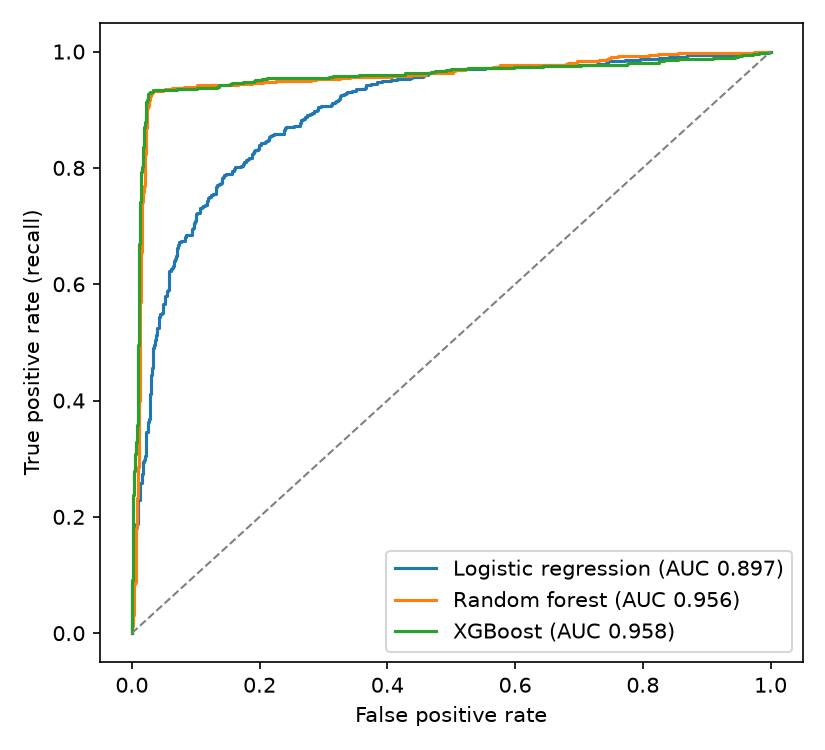
\includegraphics[width=0.55\linewidth]{figures/roc_comparison.png}
  \caption{ROC curves from out-of-fold predictions (legend: mean AUC over outer folds).}
  \label{fig:roc}
\end{figure}

\subsection{Screening operating point}
Table~\ref{tab:recall} shows the results when each model's threshold is chosen, inside the training
folds, to catch at least 90\% of AD cases.

\begin{table}[H]
  \centering
  \caption{Recall-targeted threshold (target recall $\geq 0.90$, chosen inside training folds).}
  \label{tab:recall}
  \small
  \begin{tabular}{lccccc}
    \toprule
    Model & Threshold & Recall & Specificity & Precision & Accuracy \\
    \midrule
    \inputrows{tables/recall_operating_point.tex}
    \bottomrule
  \end{tabular}
\end{table}

For the tree models the target is already met at the default threshold, so the rule
changes little: for random forest the selected thresholds (about 0.49) change no prediction, and for
XGBoost the threshold rises to about 0.56, trading a little recall for specificity. Logistic regression
must lower its threshold to about 0.26 to reach the target. It then flags 28.5\% of non-AD records as
positive (specificity 0.715), against 2.3\% for XGBoost, while detecting a similar share of AD cases
(recall 0.893 versus 0.912). Used for screening, logistic regression would make roughly twelve times as
many unnecessary referrals.

\subsection{What drives the predictions}
Both model families rely on the same five features (Figure~\ref{fig:drivers}). In the
logistic regression, FunctionalAssessment, ADL and MMSE have the largest coefficients (negative: higher
scores mean lower risk) and MemoryComplaints and BehavioralProblems the largest positive ones; every
other coefficient is below 0.25 in absolute value, and the L1 penalty sets eight of them to zero. In
XGBoost the same five features account for 70.5\% of the total gain, split almost equally among the three
scores (16--17\% each). The 2024 report ranked features by split counts, which favour continuous
features; ranked by gain, the same five features lead. We do not read the small importances of lifestyle
features such as DietQuality or SleepQuality as evidence that lifestyle matters: their correlation with
the diagnosis is below 0.07 and their contribution to the model is small.

\begin{figure}[H]
  \centering
  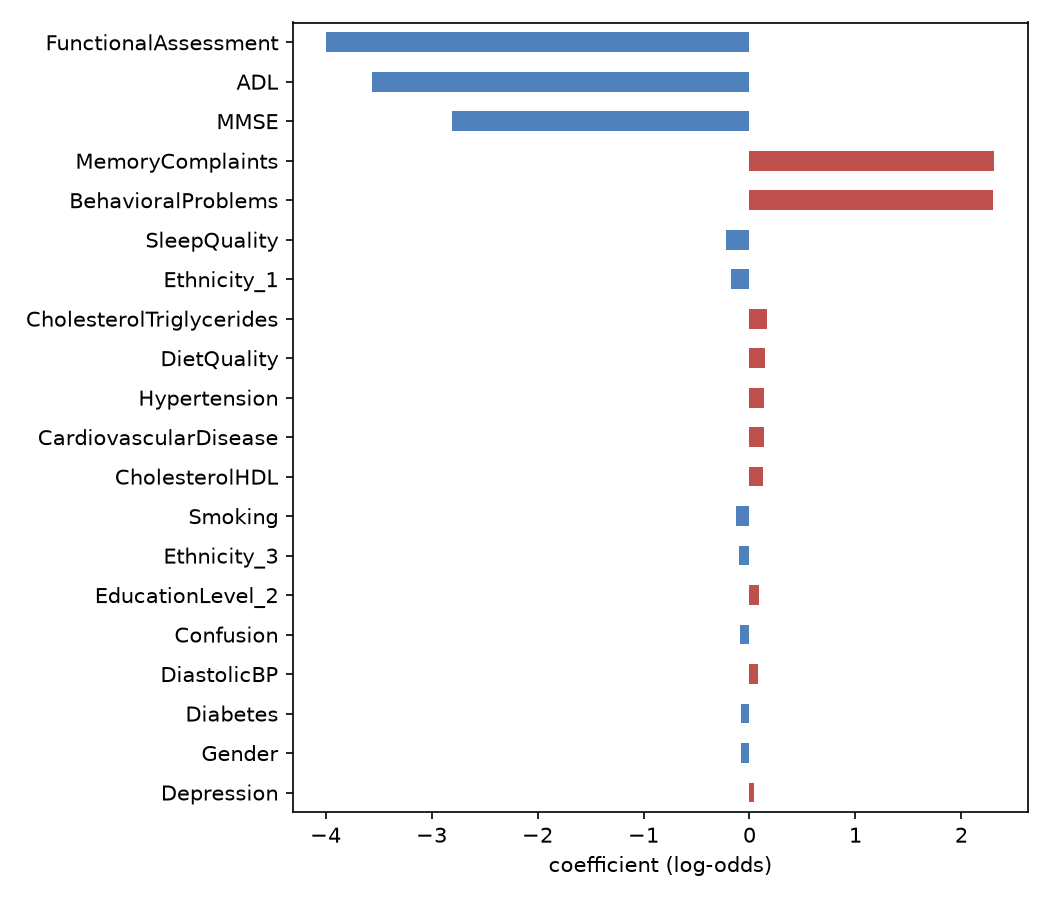
\includegraphics[width=0.48\linewidth]{figures/lr_coefficients.png}\hfill
  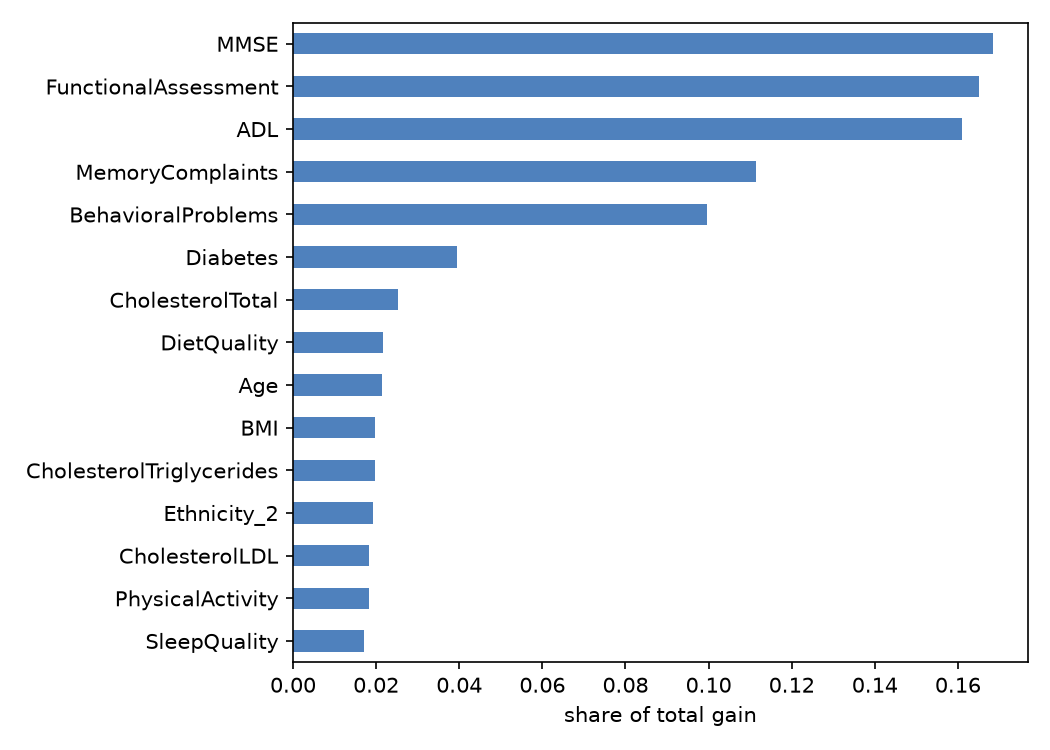
\includegraphics[width=0.48\linewidth]{figures/xgb_importance.png}
  \caption{Left: logistic regression coefficients (non-zero, largest 20). Right: XGBoost feature
  importance as share of total gain (top 15). Both from the final models fitted on all training data.}
  \label{fig:drivers}
\end{figure}

\subsection{The 2024 evaluation revisited}
\paragraph{Missing features.} Restricted to the 2024 feature set (continuous and one-hot
nominal features only), logistic regression reaches an accuracy of $0.772 \pm 0.026$ and an AUC of
$0.816 \pm 0.035$ under the same protocol. The omitted binary features are worth 6 points of accuracy.

\paragraph{Selection bias.} The 2024 XGBoost configuration (36 trees of depth 3, learning rate 0.1, row
subsampling 0.9, column subsampling 0.85) reaches 0.957 on the 2024 validation split with the current
xgboost version (0.965 was reported with an older version), but $0.952 \pm 0.006$ under 5-fold
cross-validation on the outer folds used here, with fold accuracies between 0.947 and 0.960. The model
tuned in this revision is slightly better ($0.957 \pm 0.009$), and its estimate is not affected by the
selection.

\paragraph{Kaggle.} The 2024 submission scored 0.952 on the public and 0.910 on the private
leaderboard. The public score matches the cross-validated accuracy of that configuration (0.952),
not the reported 0.965. The private score is below every outer-fold accuracy, and we cannot explain the
drop without the private labels. The 2024 report attributed it to a difference in distribution, but the
labelled and unlabelled records have nearly identical feature distributions (the largest standardized
mean difference is 0.10).

\section{Discussion}
\paragraph{Interpretability and performance.} Logistic regression identifies the right
features, and its coefficients are easy to read, but its linear form cannot represent the step-shaped
effects of MMSE, FunctionalAssessment and ADL, so it trails the tree ensembles by about 12 points of
accuracy. The selected XGBoost model uses trees of depth 2, so each tree combines at most two features;
together with Figure~\ref{fig:steps} this suggests that the structure of the data is close to additive in
a few step functions. A logistic regression on binned versions of the three scores might therefore close
much of the gap while remaining interpretable. We did not test this, because cut-offs found by inspecting
all training data would bias the evaluation; they would have to be learned inside the folds.

\paragraph{Screening.} For a screening tool, the relevant comparison is the false-positive rate at a
fixed, high recall. At a recall of about 0.9, XGBoost flags 2.3\% of non-AD records and logistic
regression 28.5\%. Random forest performs as well as XGBoost and would be an equally good choice.

\paragraph{Limitations.} The dataset is synthetic, so none of these findings is clinical evidence: the
sharp cut-off at MMSE~$=24$, a commonly used clinical threshold, most likely reflects how the generator
was built rather than how cognition declines. With 1,504 records the fold-to-fold standard deviation of
accuracy is about one point, so differences of that size, such as the one between XGBoost and random
forest, are not meaningful. The revised models' Kaggle predictions have not been scored. Finally, the
confidently misclassified records suggest a ceiling on accuracy with these features; the meta-model for
``hard'' cases proposed in the 2024 report would have to overcome labels that look unexplainable.

\paragraph{Conclusion.} Tree ensembles are clearly better than logistic regression on these data, with a
cross-validated accuracy of about 0.955 against 0.833, and far fewer false referrals at a screening threshold.
The advantage comes from the step-shaped effects of three cognitive and functional scores, which a linear
model cannot represent. The 2024 report reached the same ranking, but overstated XGBoost's accuracy and
understated logistic regression's, and explained the difference incorrectly.

\section{Changes from the submitted version}\label{sec:changes}
The version submitted in December 2024 is kept unchanged, apart from redacted student numbers, as
\texttt{report/submitted\_2024.pdf}. This revision corrects the following problems in it.
\begin{enumerate}
  \item \textbf{Logistic regression omitted all 15 binary features.} The 2024 notebook built the
  design matrix from the continuous and one-hot nominal features only, dropping MemoryComplaints,
  BehavioralProblems and the other binary features, although the report states they were used.
  \item \textbf{The logistic regression confusion matrix was mislabelled.} The notebook read
  scikit-learn's confusion matrix with the true-negative cell as the true-positive count. The reported
  precision (0.906), false-positive rate (0.235) and false-negative rate (0.211) were in fact the
  specificity, false discovery rate and false omission rate; the actual values were 0.766, 0.094 and
  0.442. The abstract's claim of a precision above 90\% was therefore wrong.
  \item \textbf{Logistic regression was evaluated on its own training data}, while XGBoost was evaluated
  on a validation split, so the two were not compared on equal terms.
  \item \textbf{The XGBoost accuracy of 96.5\% was optimistically biased.} It was the best of 32,000
  configurations on a single validation split, reported on that same split (and the split ratio itself
  was chosen by trying several). Section~\ref{sec:results} gives an estimate free of this selection bias.
  \item \textbf{The explanation of logistic regression's weakness was wrong.} The 2024 report blamed
  multicollinearity among MemoryComplaints, DifficultyCompletingTasks and Forgetfulness; those features
  were not in the model, and they are essentially uncorrelated. The actual reasons are the missing
  features and the step-shaped effects described in Section~\ref{sec:data}.
  \item \textbf{The threshold reasoning was reversed.} The 2024 report required a precision above 90\%
  in order to reduce false negatives; precision controls false positives. Missed cases are controlled by
  recall, which is what the screening threshold here targets.
  \item \textbf{The final XGBoost model was trained on 75\% of the data} and never refitted on all
  labelled records before predicting the test set.
  \item \textbf{The synthetic nature of the data was not mentioned.} Clinical interpretations in the
  2024 report should be read as statements about the data generator.
  \item \textbf{Smaller issues:} the dataset citation (now \citealp{elkharoua2024dataset}); the count of
  binary features (15, not 17, which included the target and the constant column); the title of the
  numerical summary table; the definition of the target as ``what the model predicts'' rather than the
  recorded diagnosis; and the attribution of the public/private Kaggle gap to a distribution difference,
  which the feature distributions do not support (Section~\ref{sec:results}).
\end{enumerate}
The code was rewritten accordingly: all notebooks share one preprocessing and evaluation module
(\texttt{notebooks/common.py}), and the tables and figures in this report are generated by the notebooks.

\bibliographystyle{plainnat}
\bibliography{references}

\end{document}
